\documentclass[twoside]{book}

% Packages required by doxygen
\usepackage{calc}
\usepackage{doxygen}
\usepackage{graphicx}
\usepackage[utf8]{inputenc}
\usepackage{makeidx}
\usepackage{multicol}
\usepackage{multirow}
\usepackage{textcomp}
\usepackage[table]{xcolor}

% Font selection
\usepackage[T1]{fontenc}
\usepackage{mathptmx}
\usepackage[scaled=.90]{helvet}
\usepackage{courier}
\usepackage{amssymb}
\usepackage{sectsty}
\renewcommand{\familydefault}{\sfdefault}
\allsectionsfont{%
  \fontseries{bc}\selectfont%
  \color{darkgray}%
}
\renewcommand{\DoxyLabelFont}{%
  \fontseries{bc}\selectfont%
  \color{darkgray}%
}

% Page & text layout
\usepackage{geometry}
\geometry{%
  a4paper,%
  top=2.5cm,%
  bottom=2.5cm,%
  left=2.5cm,%
  right=2.5cm%
}
\tolerance=750
\hfuzz=15pt
\hbadness=750
\setlength{\emergencystretch}{15pt}
\setlength{\parindent}{0cm}
\setlength{\parskip}{0.2cm}
\makeatletter
\renewcommand{\paragraph}{%
  \@startsection{paragraph}{4}{0ex}{-1.0ex}{1.0ex}{%
    \normalfont\normalsize\bfseries\SS@parafont%
  }%
}
\renewcommand{\subparagraph}{%
  \@startsection{subparagraph}{5}{0ex}{-1.0ex}{1.0ex}{%
    \normalfont\normalsize\bfseries\SS@subparafont%
  }%
}
\makeatother

% Headers & footers
\usepackage{fancyhdr}
\pagestyle{fancyplain}
\fancyhead[LE]{\fancyplain{}{\bfseries\thepage}}
\fancyhead[CE]{\fancyplain{}{}}
\fancyhead[RE]{\fancyplain{}{\bfseries\leftmark}}
\fancyhead[LO]{\fancyplain{}{\bfseries\rightmark}}
\fancyhead[CO]{\fancyplain{}{}}
\fancyhead[RO]{\fancyplain{}{\bfseries\thepage}}
\fancyfoot[LE]{\fancyplain{}{}}
\fancyfoot[CE]{\fancyplain{}{}}
\fancyfoot[RE]{\fancyplain{}{\bfseries\scriptsize Generated on Sat Jan 27 2018 20\-:58\-:26 for My Project by Doxygen }}
\fancyfoot[LO]{\fancyplain{}{\bfseries\scriptsize Generated on Sat Jan 27 2018 20\-:58\-:26 for My Project by Doxygen }}
\fancyfoot[CO]{\fancyplain{}{}}
\fancyfoot[RO]{\fancyplain{}{}}
\renewcommand{\footrulewidth}{0.4pt}
\renewcommand{\chaptermark}[1]{%
  \markboth{#1}{}%
}
\renewcommand{\sectionmark}[1]{%
  \markright{\thesection\ #1}%
}

% Indices & bibliography
\usepackage{natbib}
\usepackage[titles]{tocloft}
\setcounter{tocdepth}{3}
\setcounter{secnumdepth}{5}
\makeindex

% Hyperlinks (required, but should be loaded last)
\usepackage{ifpdf}
\ifpdf
  \usepackage[pdftex,pagebackref=true]{hyperref}
\else
  \usepackage[ps2pdf,pagebackref=true]{hyperref}
\fi
\hypersetup{%
  colorlinks=true,%
  linkcolor=blue,%
  citecolor=blue,%
  unicode%
}

% Custom commands
\newcommand{\clearemptydoublepage}{%
  \newpage{\pagestyle{empty}\cleardoublepage}%
}


%===== C O N T E N T S =====

\begin{document}

% Titlepage & ToC
\hypersetup{pageanchor=false}
\pagenumbering{roman}
\begin{titlepage}
\vspace*{7cm}
\begin{center}%
{\Large My Project }\\
\vspace*{1cm}
{\large Generated by Doxygen 1.8.6}\\
\vspace*{0.5cm}
{\small Sat Jan 27 2018 20:58:26}\\
\end{center}
\end{titlepage}
\clearemptydoublepage
\tableofcontents
\clearemptydoublepage
\pagenumbering{arabic}
\hypersetup{pageanchor=true}

%--- Begin generated contents ---
\chapter{Class Index}
\section{Class List}
Here are the classes, structs, unions and interfaces with brief descriptions\-:\begin{DoxyCompactList}
\item\contentsline{section}{\hyperlink{classis__container}{is\-\_\-container$<$ T $>$} }{\pageref{classis__container}}{}
\item\contentsline{section}{\hyperlink{structiterate__tuple}{iterate\-\_\-tuple$<$ is\-\_\-same\-\_\-type, index, Printer, Args $>$} }{\pageref{structiterate__tuple}}{}
\item\contentsline{section}{\hyperlink{structiterate__tuple_3_01false_00_01index_00_01_printer_00_01_args_8_8_8_4}{iterate\-\_\-tuple$<$ false, index, Printer, Args...$>$} }{\pageref{structiterate__tuple_3_01false_00_01index_00_01_printer_00_01_args_8_8_8_4}}{}
\item\contentsline{section}{\hyperlink{structiterate__tuple_3_01state_00_010_00_01_printer_00_01_args_8_8_8_4}{iterate\-\_\-tuple$<$ state, 0, Printer, Args...$>$} }{\pageref{structiterate__tuple_3_01state_00_010_00_01_printer_00_01_args_8_8_8_4}}{}
\item\contentsline{section}{\hyperlink{structt__printer}{t\-\_\-printer} }{\pageref{structt__printer}}{}
\end{DoxyCompactList}

\chapter{File Index}
\section{File List}
Here is a list of all files with brief descriptions\-:\begin{DoxyCompactList}
\item\contentsline{section}{\hyperlink{document_8h}{document.\-h} }{\pageref{document_8h}}{}
\item\contentsline{section}{\hyperlink{main_8cpp}{main.\-cpp} }{\pageref{main_8cpp}}{}
\item\contentsline{section}{\hyperlink{shape_8h}{shape.\-h} }{\pageref{shape_8h}}{}
\item\contentsline{section}{\hyperlink{version_8h}{version.\-h} }{\pageref{version_8h}}{}
\end{DoxyCompactList}

\chapter{Class Documentation}
\hypertarget{classis__container}{\section{is\-\_\-container$<$ T $>$ Class Template Reference}
\label{classis__container}\index{is\-\_\-container$<$ T $>$@{is\-\_\-container$<$ T $>$}}
}


{\ttfamily \#include $<$check\-\_\-type.\-h$>$}

\subsection*{Static Public Attributes}
\begin{DoxyCompactItemize}
\item 
static constexpr auto \hyperlink{classis__container_ac4653fd3cc2c8268f003fbe2d878d48e}{value} = has\-\_\-iterator$<$T$>$(nullptr)
\end{DoxyCompactItemize}


\subsection{Member Data Documentation}
\hypertarget{classis__container_ac4653fd3cc2c8268f003fbe2d878d48e}{\index{is\-\_\-container@{is\-\_\-container}!value@{value}}
\index{value@{value}!is_container@{is\-\_\-container}}
\subsubsection[{value}]{\setlength{\rightskip}{0pt plus 5cm}template$<$typename T $>$ constexpr auto {\bf is\-\_\-container}$<$ T $>$\-::value = has\-\_\-iterator$<$T$>$(nullptr)\hspace{0.3cm}{\ttfamily [static]}}}\label{classis__container_ac4653fd3cc2c8268f003fbe2d878d48e}


The documentation for this class was generated from the following file\-:\begin{DoxyCompactItemize}
\item 
\hyperlink{check__type_8h}{check\-\_\-type.\-h}\end{DoxyCompactItemize}

\hypertarget{structiterate__tuple}{\section{iterate\-\_\-tuple$<$ is\-\_\-same\-\_\-type, index, Printer, Args $>$ Struct Template Reference}
\label{structiterate__tuple}\index{iterate\-\_\-tuple$<$ is\-\_\-same\-\_\-type, index, Printer, Args $>$@{iterate\-\_\-tuple$<$ is\-\_\-same\-\_\-type, index, Printer, Args $>$}}
}


{\ttfamily \#include $<$print\-\_\-tuple.\-h$>$}

\subsection*{Static Public Member Functions}
\begin{DoxyCompactItemize}
\item 
static bool \hyperlink{structiterate__tuple_ae1b406f4288f5d13606983d14a251ca2}{next} (std\-::tuple$<$ Args...$>$ \&t, Printer \hyperlink{structprinter}{printer})
\end{DoxyCompactItemize}


\subsection{Member Function Documentation}
\hypertarget{structiterate__tuple_ae1b406f4288f5d13606983d14a251ca2}{\index{iterate\-\_\-tuple@{iterate\-\_\-tuple}!next@{next}}
\index{next@{next}!iterate_tuple@{iterate\-\_\-tuple}}
\subsubsection[{next}]{\setlength{\rightskip}{0pt plus 5cm}template$<$bool is\-\_\-same\-\_\-type, int index, typename Printer , typename... Args$>$ static bool {\bf iterate\-\_\-tuple}$<$ is\-\_\-same\-\_\-type, index, Printer, Args $>$\-::next (
\begin{DoxyParamCaption}
\item[{std\-::tuple$<$ Args...$>$ \&}]{t, }
\item[{Printer}]{printer}
\end{DoxyParamCaption}
)\hspace{0.3cm}{\ttfamily [inline]}, {\ttfamily [static]}}}\label{structiterate__tuple_ae1b406f4288f5d13606983d14a251ca2}


The documentation for this struct was generated from the following file\-:\begin{DoxyCompactItemize}
\item 
\hyperlink{print__tuple_8h}{print\-\_\-tuple.\-h}\end{DoxyCompactItemize}

\hypertarget{structiterate__tuple_3_01false_00_01index_00_01_printer_00_01_args_8_8_8_4}{\section{iterate\-\_\-tuple$<$ false, index, Printer, Args...$>$ Struct Template Reference}
\label{structiterate__tuple_3_01false_00_01index_00_01_printer_00_01_args_8_8_8_4}\index{iterate\-\_\-tuple$<$ false, index, Printer, Args...$>$@{iterate\-\_\-tuple$<$ false, index, Printer, Args...$>$}}
}


{\ttfamily \#include $<$print\-\_\-tuple.\-h$>$}

\subsection*{Static Public Member Functions}
\begin{DoxyCompactItemize}
\item 
static bool \hyperlink{structiterate__tuple_3_01false_00_01index_00_01_printer_00_01_args_8_8_8_4_a82039badb01003122f02001984aa23d7}{next} (std\-::tuple$<$ Args...$>$ \&t, Printer \hyperlink{structprinter}{printer})
\end{DoxyCompactItemize}


\subsection{Member Function Documentation}
\hypertarget{structiterate__tuple_3_01false_00_01index_00_01_printer_00_01_args_8_8_8_4_a82039badb01003122f02001984aa23d7}{\index{iterate\-\_\-tuple$<$ false, index, Printer, Args...$>$@{iterate\-\_\-tuple$<$ false, index, Printer, Args...$>$}!next@{next}}
\index{next@{next}!iterate_tuple< false, index, Printer, Args...>@{iterate\-\_\-tuple$<$ false, index, Printer, Args...$>$}}
\subsubsection[{next}]{\setlength{\rightskip}{0pt plus 5cm}template$<$int index, typename Printer , typename... Args$>$ static bool {\bf iterate\-\_\-tuple}$<$ false, index, Printer, Args...$>$\-::next (
\begin{DoxyParamCaption}
\item[{std\-::tuple$<$ Args...$>$ \&}]{t, }
\item[{Printer}]{printer}
\end{DoxyParamCaption}
)\hspace{0.3cm}{\ttfamily [inline]}, {\ttfamily [static]}}}\label{structiterate__tuple_3_01false_00_01index_00_01_printer_00_01_args_8_8_8_4_a82039badb01003122f02001984aa23d7}


The documentation for this struct was generated from the following file\-:\begin{DoxyCompactItemize}
\item 
\hyperlink{print__tuple_8h}{print\-\_\-tuple.\-h}\end{DoxyCompactItemize}

\hypertarget{structiterate__tuple_3_01state_00_010_00_01_printer_00_01_args_8_8_8_4}{\section{iterate\-\_\-tuple$<$ state, 0, Printer, Args...$>$ Struct Template Reference}
\label{structiterate__tuple_3_01state_00_010_00_01_printer_00_01_args_8_8_8_4}\index{iterate\-\_\-tuple$<$ state, 0, Printer, Args...$>$@{iterate\-\_\-tuple$<$ state, 0, Printer, Args...$>$}}
}


{\ttfamily \#include $<$print\-\_\-tuple.\-h$>$}

\subsection*{Static Public Member Functions}
\begin{DoxyCompactItemize}
\item 
static bool \hyperlink{structiterate__tuple_3_01state_00_010_00_01_printer_00_01_args_8_8_8_4_a1bae83d8d5bca2fb671097da75975e4a}{next} (std\-::tuple$<$ Args...$>$ \&t, Printer printer)
\end{DoxyCompactItemize}


\subsection{Member Function Documentation}
\hypertarget{structiterate__tuple_3_01state_00_010_00_01_printer_00_01_args_8_8_8_4_a1bae83d8d5bca2fb671097da75975e4a}{\index{iterate\-\_\-tuple$<$ state, 0, Printer, Args...$>$@{iterate\-\_\-tuple$<$ state, 0, Printer, Args...$>$}!next@{next}}
\index{next@{next}!iterate_tuple< state, 0, Printer, Args...>@{iterate\-\_\-tuple$<$ state, 0, Printer, Args...$>$}}
\subsubsection[{next}]{\setlength{\rightskip}{0pt plus 5cm}template$<$bool state, typename Printer , typename... Args$>$ static bool {\bf iterate\-\_\-tuple}$<$ state, 0, Printer, Args...$>$\-::next (
\begin{DoxyParamCaption}
\item[{std\-::tuple$<$ Args...$>$ \&}]{t, }
\item[{Printer}]{printer}
\end{DoxyParamCaption}
)\hspace{0.3cm}{\ttfamily [inline]}, {\ttfamily [static]}}}\label{structiterate__tuple_3_01state_00_010_00_01_printer_00_01_args_8_8_8_4_a1bae83d8d5bca2fb671097da75975e4a}


The documentation for this struct was generated from the following file\-:\begin{DoxyCompactItemize}
\item 
\hyperlink{print__tuple_8h}{print\-\_\-tuple.\-h}\end{DoxyCompactItemize}

\hypertarget{structprinter}{\section{printer Struct Reference}
\label{structprinter}\index{printer@{printer}}
}
\subsection*{Public Member Functions}
\begin{DoxyCompactItemize}
\item 
{\footnotesize template$<$typename T $>$ }\\void \hyperlink{structprinter_a493ea296fb0a66f6ff5002c1506359d8}{operator()} (T \&\&t, int index)
\end{DoxyCompactItemize}


\subsection{Detailed Description}
Печатает элементы ip адреса 
\begin{DoxyParams}[1]{Parameters}
\mbox{\tt in}  & {\em T\&\&} & Объект, который нужно распечатать \\
\hline
\mbox{\tt in}  & {\em index} & Число, указывающее, стоит ли этот элемент в начале адреса или нет \\
\hline
\end{DoxyParams}


\subsection{Member Function Documentation}
\hypertarget{structprinter_a493ea296fb0a66f6ff5002c1506359d8}{\index{printer@{printer}!operator()@{operator()}}
\index{operator()@{operator()}!printer@{printer}}
\subsubsection[{operator()}]{\setlength{\rightskip}{0pt plus 5cm}template$<$typename T $>$ void printer\-::operator() (
\begin{DoxyParamCaption}
\item[{T \&\&}]{t, }
\item[{int}]{index}
\end{DoxyParamCaption}
)\hspace{0.3cm}{\ttfamily [inline]}}}\label{structprinter_a493ea296fb0a66f6ff5002c1506359d8}


The documentation for this struct was generated from the following file\-:\begin{DoxyCompactItemize}
\item 
\hyperlink{main_8cpp}{main.\-cpp}\end{DoxyCompactItemize}

\chapter{File Documentation}
\hypertarget{check__type_8h}{\section{check\-\_\-type.\-h File Reference}
\label{check__type_8h}\index{check\-\_\-type.\-h@{check\-\_\-type.\-h}}
}
This graph shows which files directly or indirectly include this file\-:
\nopagebreak
\begin{figure}[H]
\begin{center}
\leavevmode
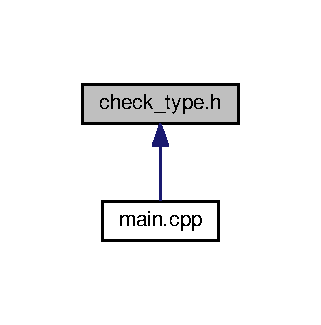
\includegraphics[width=154pt]{check__type_8h__dep__incl}
\end{center}
\end{figure}
\subsection*{Classes}
\begin{DoxyCompactItemize}
\item 
class \hyperlink{classis__container}{is\-\_\-container$<$ T $>$}
\end{DoxyCompactItemize}

\hypertarget{main_8cpp}{\section{main.\-cpp File Reference}
\label{main_8cpp}\index{main.\-cpp@{main.\-cpp}}
}
{\ttfamily \#include $<$iostream$>$}\\*
{\ttfamily \#include $<$utility$>$}\\*
{\ttfamily \#include $<$tuple$>$}\\*
{\ttfamily \#include $<$bitset$>$}\\*
{\ttfamily \#include $<$vector$>$}\\*
{\ttfamily \#include $<$list$>$}\\*
{\ttfamily \#include $<$functional$>$}\\*
{\ttfamily \#include \char`\"{}check\-\_\-type.\-h\char`\"{}}\\*
{\ttfamily \#include \char`\"{}print\-\_\-tuple.\-h\char`\"{}}\\*
Include dependency graph for main.\-cpp\-:
\nopagebreak
\begin{figure}[H]
\begin{center}
\leavevmode
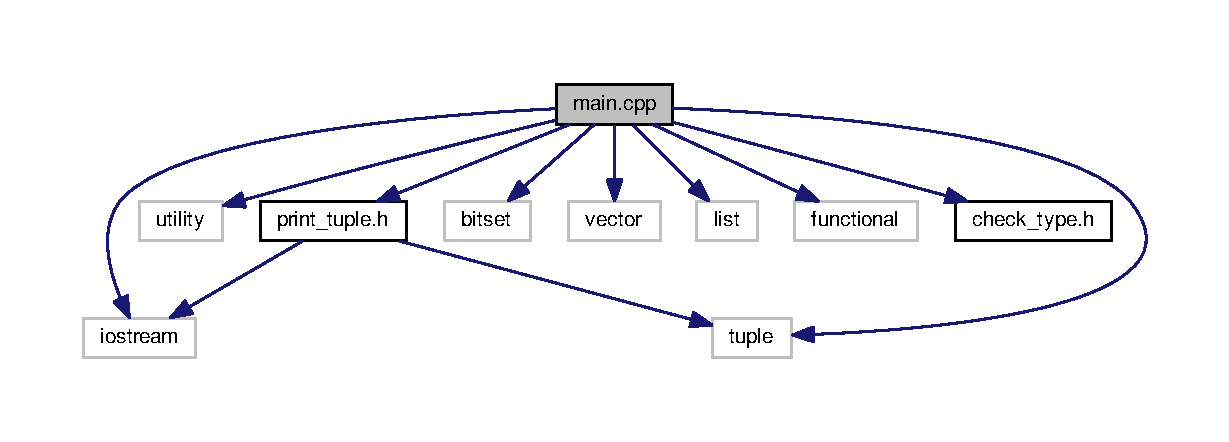
\includegraphics[width=350pt]{main_8cpp__incl}
\end{center}
\end{figure}
\subsection*{Classes}
\begin{DoxyCompactItemize}
\item 
struct \hyperlink{structprinter}{printer}
\end{DoxyCompactItemize}
\subsection*{Functions}
\begin{DoxyCompactItemize}
\item 
{\footnotesize template$<$typename T , typename Printer $>$ }\\void \hyperlink{main_8cpp_a2e507a49231a92dd51a74153d941a10b}{print} (T \&\&t, Printer \hyperlink{structprinter}{printer}, int)
\item 
{\footnotesize template$<$typename T , typename Printer $>$ }\\void \hyperlink{main_8cpp_a4d92f34c852cf08c698ce9ff9b8f40e1}{print} (T \&\&t, Printer \hyperlink{structprinter}{printer}, char)
\item 
{\footnotesize template$<$typename Printer $>$ }\\void \hyperlink{main_8cpp_a650caaec23d14a266eb863256c192da2}{print} (std\-::string t, Printer, char)
\item 
{\footnotesize template$<$typename T $>$ }\\void \hyperlink{main_8cpp_a5a2ed2f3cccd43a84bfd7d2740475be1}{print\-\_\-ip} (T \&\&t)
\item 
{\footnotesize template$<$typename... Args$>$ }\\void \hyperlink{main_8cpp_adf6cb0a6bc6c2be1c8468b73110978ba}{print\-\_\-ip} (std\-::tuple$<$ Args...$>$ t)
\item 
int \hyperlink{main_8cpp_ae66f6b31b5ad750f1fe042a706a4e3d4}{main} ()
\end{DoxyCompactItemize}


\subsection{Function Documentation}
\hypertarget{main_8cpp_ae66f6b31b5ad750f1fe042a706a4e3d4}{\index{main.\-cpp@{main.\-cpp}!main@{main}}
\index{main@{main}!main.cpp@{main.\-cpp}}
\subsubsection[{main}]{\setlength{\rightskip}{0pt plus 5cm}int main (
\begin{DoxyParamCaption}
{}
\end{DoxyParamCaption}
)}}\label{main_8cpp_ae66f6b31b5ad750f1fe042a706a4e3d4}
\hypertarget{main_8cpp_a2e507a49231a92dd51a74153d941a10b}{\index{main.\-cpp@{main.\-cpp}!print@{print}}
\index{print@{print}!main.cpp@{main.\-cpp}}
\subsubsection[{print}]{\setlength{\rightskip}{0pt plus 5cm}template$<$typename T , typename Printer $>$ void print (
\begin{DoxyParamCaption}
\item[{T \&\&}]{t, }
\item[{Printer}]{printer, }
\item[{int}]{}
\end{DoxyParamCaption}
)}}\label{main_8cpp_a2e507a49231a92dd51a74153d941a10b}
Обработка целочисленных типов 
\begin{DoxyParams}[1]{Parameters}
\mbox{\tt in}  & {\em T\&\&} & Объект, который нужно обработать \\
\hline
\mbox{\tt in}  & {\em int} & -\/ целочисленный тип \\
\hline
\end{DoxyParams}
\hypertarget{main_8cpp_a4d92f34c852cf08c698ce9ff9b8f40e1}{\index{main.\-cpp@{main.\-cpp}!print@{print}}
\index{print@{print}!main.cpp@{main.\-cpp}}
\subsubsection[{print}]{\setlength{\rightskip}{0pt plus 5cm}template$<$typename T , typename Printer $>$ void print (
\begin{DoxyParamCaption}
\item[{T \&\&}]{t, }
\item[{Printer}]{printer, }
\item[{char}]{}
\end{DoxyParamCaption}
)}}\label{main_8cpp_a4d92f34c852cf08c698ce9ff9b8f40e1}
Обработка контейнерных типов 
\begin{DoxyParams}[1]{Parameters}
\mbox{\tt in}  & {\em T\&\&} & Объект, который нужно обработать \\
\hline
\mbox{\tt in}  & {\em char} & -\/ контейнерный тип \\
\hline
\end{DoxyParams}
\hypertarget{main_8cpp_a650caaec23d14a266eb863256c192da2}{\index{main.\-cpp@{main.\-cpp}!print@{print}}
\index{print@{print}!main.cpp@{main.\-cpp}}
\subsubsection[{print}]{\setlength{\rightskip}{0pt plus 5cm}template$<$typename Printer $>$ void print (
\begin{DoxyParamCaption}
\item[{std\-::string}]{t, }
\item[{Printer}]{, }
\item[{char}]{}
\end{DoxyParamCaption}
)}}\label{main_8cpp_a650caaec23d14a266eb863256c192da2}
Обработка строк 
\begin{DoxyParams}[1]{Parameters}
\mbox{\tt in}  & {\em std\-::string} & строка, которую нужно обработать \\
\hline
\mbox{\tt in}  & {\em int} & -\/ char -\/ контейнерный тип \\
\hline
\end{DoxyParams}
\hypertarget{main_8cpp_a5a2ed2f3cccd43a84bfd7d2740475be1}{\index{main.\-cpp@{main.\-cpp}!print\-\_\-ip@{print\-\_\-ip}}
\index{print\-\_\-ip@{print\-\_\-ip}!main.cpp@{main.\-cpp}}
\subsubsection[{print\-\_\-ip}]{\setlength{\rightskip}{0pt plus 5cm}template$<$typename T $>$ void print\-\_\-ip (
\begin{DoxyParamCaption}
\item[{T \&\&}]{t}
\end{DoxyParamCaption}
)}}\label{main_8cpp_a5a2ed2f3cccd43a84bfd7d2740475be1}
Отделяет контейнеры от целочисленных типов 
\begin{DoxyParams}[1]{Parameters}
\mbox{\tt in}  & {\em T\&\&} & Объект, который нужно обработать \\
\hline
\end{DoxyParams}
\hypertarget{main_8cpp_adf6cb0a6bc6c2be1c8468b73110978ba}{\index{main.\-cpp@{main.\-cpp}!print\-\_\-ip@{print\-\_\-ip}}
\index{print\-\_\-ip@{print\-\_\-ip}!main.cpp@{main.\-cpp}}
\subsubsection[{print\-\_\-ip}]{\setlength{\rightskip}{0pt plus 5cm}template$<$typename... Args$>$ void print\-\_\-ip (
\begin{DoxyParamCaption}
\item[{std\-::tuple$<$ Args...$>$}]{t}
\end{DoxyParamCaption}
)}}\label{main_8cpp_adf6cb0a6bc6c2be1c8468b73110978ba}
Отдельная специализация для кортежа 
\hypertarget{print__tuple_8h}{\section{print\-\_\-tuple.\-h File Reference}
\label{print__tuple_8h}\index{print\-\_\-tuple.\-h@{print\-\_\-tuple.\-h}}
}
{\ttfamily \#include $<$tuple$>$}\\*
{\ttfamily \#include $<$iostream$>$}\\*
Include dependency graph for print\-\_\-tuple.\-h\-:
\nopagebreak
\begin{figure}[H]
\begin{center}
\leavevmode
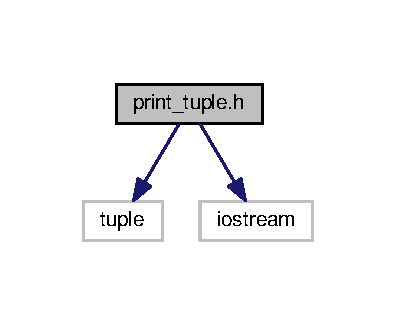
\includegraphics[width=190pt]{print__tuple_8h__incl}
\end{center}
\end{figure}
This graph shows which files directly or indirectly include this file\-:
\nopagebreak
\begin{figure}[H]
\begin{center}
\leavevmode
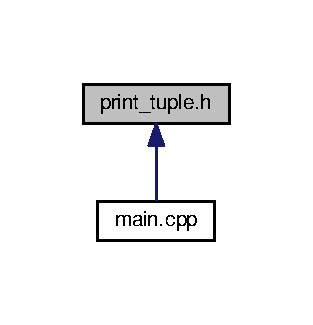
\includegraphics[width=150pt]{print__tuple_8h__dep__incl}
\end{center}
\end{figure}
\subsection*{Classes}
\begin{DoxyCompactItemize}
\item 
struct \hyperlink{structiterate__tuple}{iterate\-\_\-tuple$<$ is\-\_\-same\-\_\-type, index, Printer, Args $>$}
\item 
struct \hyperlink{structiterate__tuple_3_01state_00_010_00_01_printer_00_01_args_8_8_8_4}{iterate\-\_\-tuple$<$ state, 0, Printer, Args...$>$}
\item 
struct \hyperlink{structiterate__tuple_3_01false_00_01index_00_01_printer_00_01_args_8_8_8_4}{iterate\-\_\-tuple$<$ false, index, Printer, Args...$>$}
\end{DoxyCompactItemize}
\subsection*{Functions}
\begin{DoxyCompactItemize}
\item 
{\footnotesize template$<$typename Printer , typename... Args$>$ }\\void \hyperlink{print__tuple_8h_ad92b0d65b0af48e2ba53b01111bea131}{print\-\_\-tuple} (std\-::tuple$<$ Args...$>$ \&t, Printer printer)
\end{DoxyCompactItemize}


\subsection{Function Documentation}
\hypertarget{print__tuple_8h_ad92b0d65b0af48e2ba53b01111bea131}{\index{print\-\_\-tuple.\-h@{print\-\_\-tuple.\-h}!print\-\_\-tuple@{print\-\_\-tuple}}
\index{print\-\_\-tuple@{print\-\_\-tuple}!print_tuple.h@{print\-\_\-tuple.\-h}}
\subsubsection[{print\-\_\-tuple}]{\setlength{\rightskip}{0pt plus 5cm}template$<$typename Printer , typename... Args$>$ void print\-\_\-tuple (
\begin{DoxyParamCaption}
\item[{std\-::tuple$<$ Args...$>$ \&}]{t, }
\item[{Printer}]{printer}
\end{DoxyParamCaption}
)}}\label{print__tuple_8h_ad92b0d65b0af48e2ba53b01111bea131}
Рекурсивный обход кортежа с печатью элементов
\begin{DoxyItemize}
\item прямой проход -\/ проверка типов
\item обратный проход -\/ печать элементов 
\end{DoxyItemize}
\hypertarget{version_8h}{\section{version.\-h File Reference}
\label{version_8h}\index{version.\-h@{version.\-h}}
}
\subsection*{Macros}
\begin{DoxyCompactItemize}
\item 
\#define \hyperlink{version_8h_a4a5fc96a4bdd7d68ed99ccce9ca2e77e}{P\-R\-O\-J\-E\-C\-T\-\_\-\-V\-E\-R\-S\-I\-O\-N\-\_\-\-P\-A\-T\-C\-H}~36
\end{DoxyCompactItemize}


\subsection{Macro Definition Documentation}
\hypertarget{version_8h_a4a5fc96a4bdd7d68ed99ccce9ca2e77e}{\index{version.\-h@{version.\-h}!P\-R\-O\-J\-E\-C\-T\-\_\-\-V\-E\-R\-S\-I\-O\-N\-\_\-\-P\-A\-T\-C\-H@{P\-R\-O\-J\-E\-C\-T\-\_\-\-V\-E\-R\-S\-I\-O\-N\-\_\-\-P\-A\-T\-C\-H}}
\index{P\-R\-O\-J\-E\-C\-T\-\_\-\-V\-E\-R\-S\-I\-O\-N\-\_\-\-P\-A\-T\-C\-H@{P\-R\-O\-J\-E\-C\-T\-\_\-\-V\-E\-R\-S\-I\-O\-N\-\_\-\-P\-A\-T\-C\-H}!version.h@{version.\-h}}
\subsubsection[{P\-R\-O\-J\-E\-C\-T\-\_\-\-V\-E\-R\-S\-I\-O\-N\-\_\-\-P\-A\-T\-C\-H}]{\setlength{\rightskip}{0pt plus 5cm}\#define P\-R\-O\-J\-E\-C\-T\-\_\-\-V\-E\-R\-S\-I\-O\-N\-\_\-\-P\-A\-T\-C\-H~36}}\label{version_8h_a4a5fc96a4bdd7d68ed99ccce9ca2e77e}

%--- End generated contents ---

% Index
\newpage
\phantomsection
\addcontentsline{toc}{chapter}{Index}
\printindex

\end{document}
